%! Author = hiros
%! Date = 2020-03-01

\title{\textbf{COSC 3p94 - Stage 1}\\\large\emph{Learning Management System Development}}

\author{Zain Alqudah\\Kyle Giammarco\\David Cheong}
\date{\textbf{\today}}

% Preamble
\documentclass[12pt]{article}
\usepackage{titlesec}
\usepackage[margin=1in]{geometry}
\usepackage{microtype}
\usepackage{fontspec}
\setmainfont[Ligatures=TeX]{Candara}
\usepackage{graphicx}
\graphicspath{ {../auxil/} }

\titleformat{\section}
{\normalfont\Large\textbf}{Section\ \thesection}{18pt}{\Large}

\titleformat{\subsection}
{\normalfont\large\emph}{\thesubsection}{16pt}{\large}

% Packages
\usepackage{amsmath}
\usepackage{hyperref}
% Document
\begin{document}

    \maketitle

    \newpage

    \tableofcontents

    \newpage


    \section{User Requirements}\label{sec:user-requirements}

    \subsection{The role of each actor}\label{subsec:the-role-of-each-actor}

    There are three main roles for each individual, student, instructor and admin.
    The actor can have any of these roles, and can have all of these roles.
    On initial setup a super admin will need to be assigned in order to give other actors their roles.
    A user is given a student role, once enrolled in a class.
    An instructor is given their role, once they are in charge of a course.
    And super admins and admins are the only ones able to give the admin role to others.

    \subsection{Security}\label{subsec:security}

    There will be a main login for the individual, with no roles presented to them until given to them by someone with more permissions.
    Instructors and Admins can make courses, and add people to those courses.
    Admins can add an individual to a course as an instructor and give admin privilages to a user.
    Admins with the permission to take away permissions from a user are denoted as SuperAdmins, and are the only ones able to demote a user.
    A user can hold many roles, and is not limited to only being a student or instructor or admin.
    A instructor can have the student role as well, as well as an admin can have instructor role as well.

    \subsection{What services are presented}\label{subsec:what-services-are-presented}

    There are many features available in modern learning management systems.
    The services present within our new implementation takes inspiration from these other solutions and intends to implement them in a more seamless manner to the end user.

    \paragraph{}
    The services are as follows (those with emphasis are most important according to our surveys):
    \begin{itemize}
        \item User - Profile
        \begin{itemize}
            \item Name
            \item Bio
            \item Settings
            \begin{itemize}
                \item Theme (Light|Dark)
                \item Font and Font Size
            \end{itemize}
            \item Date of Birth
        \end{itemize}
        \item Course
        \begin{itemize}
            \item Name
            \item Description
            \item Teachers
            \item \textbf{Assignments}
            \item \textbf{Documents}
            \item Forums
            \item Quizzes
            \item \textbf{Assignments}
            \item \textbf{Grade Reporting}
        \end{itemize}
        \item Calendar
    \end{itemize}

    \subsection{Navigation}\label{subsec:navigation}

    Navigation through the site will be mainly through a header that contains the courses the individual has access to, with sections and subsections for those courses on a sidebar.
    Settings for the individual will be accessed through the profile image on the top right.
    With more advanced administrative tools available on the right for those that have permissions.

    \subsection{User Input}\label{subsec:user-input}

    The site will be accessible through either keyboard and/or mouse, with appropriate compatibility for mobile and touch screens.

    \subsection{Personalization Tools}\label{subsec:personalization-tools}

    There will be a couple options in the way of personalization tools.
    The user will be able to choose between two preset themes, either a light theme and a dark theme.
    The font used by the website can also be chosen, from a list of preset fonts that are supported.

    \subsection{Organization and Layout}\label{subsec:organization-and-layout}

    If the user is not logged in, the site will prompt the user with a login|register screen on the right, with announcements for the school on the left.
    Once the user is logged in, they are shown a main page, similar to that of the storyboard (Section\ \ref{sec:storyboard}).
    This page links into all the main features of the site, including a calendar, access to their courses and their own profile.

    \subsection{User Experience}\label{subsec:user-experience}

    The user experience is an important factor that needs to be addressed.
    Using the feedback from the survey and empathising with the users we will be able to create a seamless experience that is pleasant to interact with.
    An HTA analysis of our own site will allow us to keep everything that is important within access, but still have an uncluttered and distraction free interface.


    \section{Existing Site Analysis}\label{sec:existing-site-analysis}

    D2L and Sakai are similar websites but have some significant design differences.
    From a visual point of view, Sakai has more of a structured approach while D2L has more of a flowing design.
    There’s much more notification icons, buttons, and progress bars in D2L which help the student figure out what assignment or course is more pressing.

    Practically, D2L and Sakai serve the same function, but they differ in how they allow the user to use those features and what kind of feedback they receive.
    Both D2L and Sakai have a profile/portfolio feature where you can add information about yourself and add others.
    That feature is not the most useful as most students will not use it.
    The D2L e-portfolio feature is a bit more practical as it allows you to show off your work rather than Sakai’s social features which only allow you to post on your wall.
    D2L allows for more personalization in terms of what data is displayed.
    Things like the calendar, announcements, and course contents are much more thorough and customizable.This makes them more useful and impactful for the user.

    Course content is compartmentalized further in D2L compared to Sakai.
    Course content, assignments, links, weekly materials, etc.\ all have their own tabs with direct links to the content, and a progress bar to show how much of that content has been consumed/finished.
    D2L also has a Quick Tools section that allows easy access to summarized information like grades and submissions.

    Other than that, the rest of the features are basically the same.
    They both have group features where you can manage and search for groups to join.
    Resources are available to users on both websites to manage and access.
    Both home menus contain an overview of all the important information for the user.


    \section{Control Map (HTA)}\label{sec:control-maphta}

    %todo David


    \section{KLM Analysis}\label{sec:klm-analysis}

    %todo David


    \section{Existing Site Critique}\label{sec:existing-site-critique}

    %todo David


    \section{Survey Results}\label{sec:survey-results}

    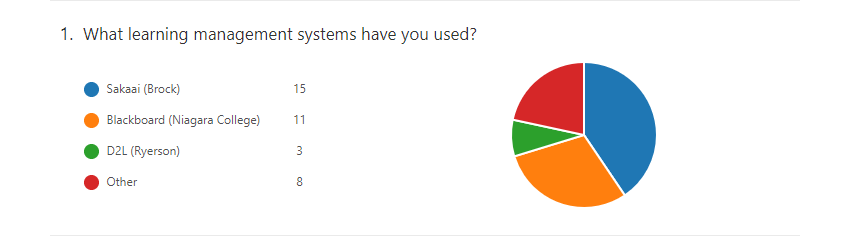
\includegraphics[width=\textwidth]{survey/1.png}
    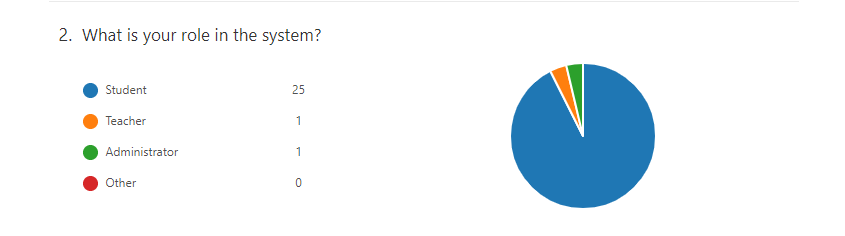
\includegraphics[width=\textwidth]{survey/2.png}
    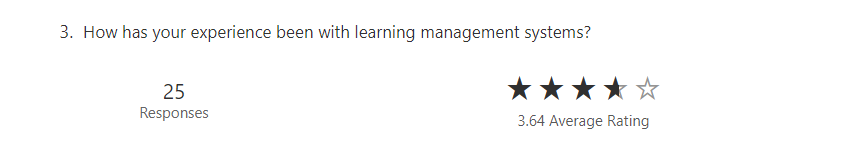
\includegraphics[width=\textwidth]{survey/3.png}
    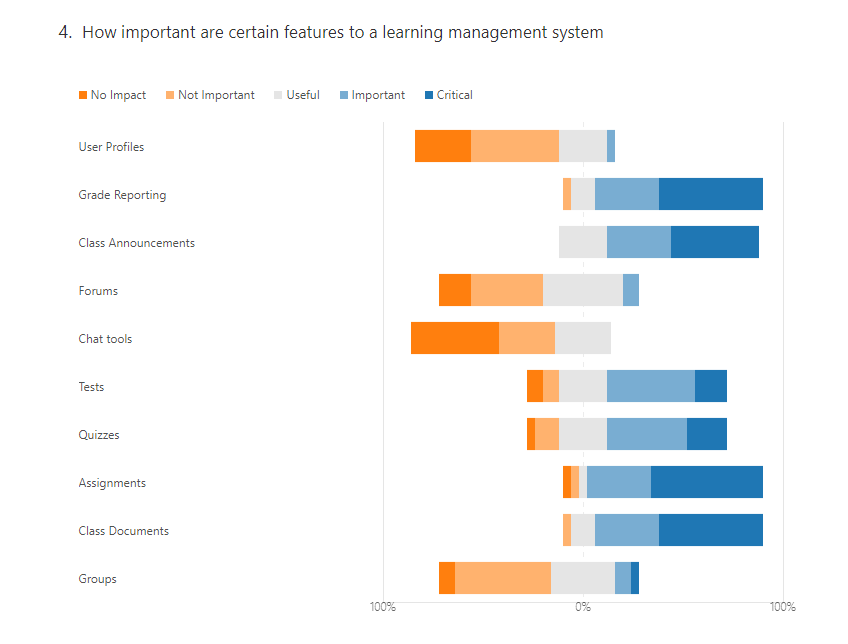
\includegraphics[width=\textwidth]{survey/4.png}
    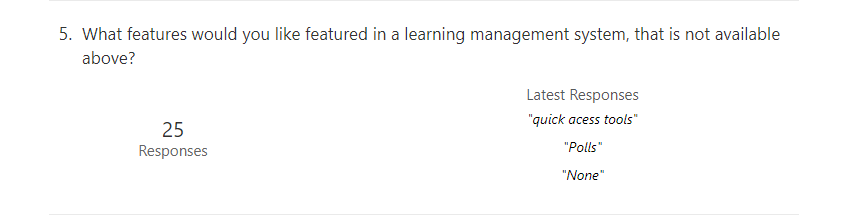
\includegraphics[width=\textwidth]{survey/5.png}
    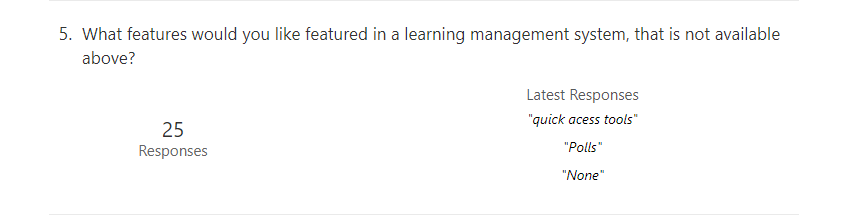
\includegraphics[width=\textwidth]{survey/6.png}
    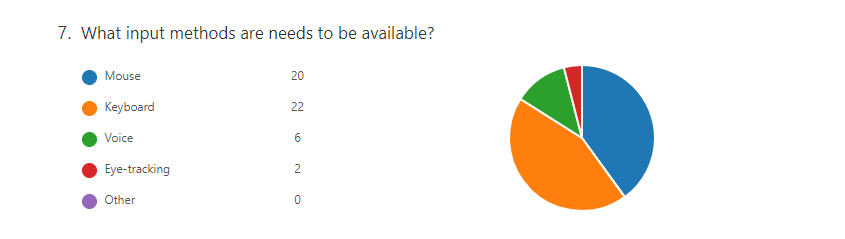
\includegraphics[width=\textwidth]{survey/7.png}
    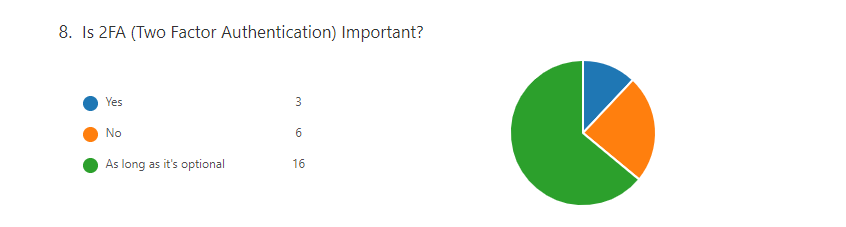
\includegraphics[width=\textwidth]{survey/8.png}
    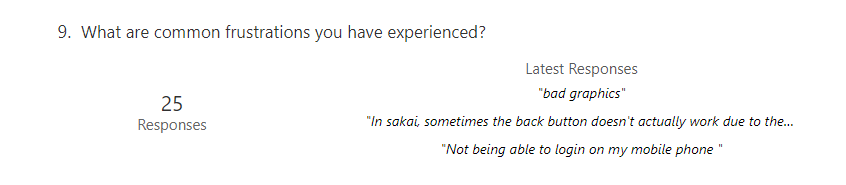
\includegraphics[width=\textwidth]{survey/9.png}
    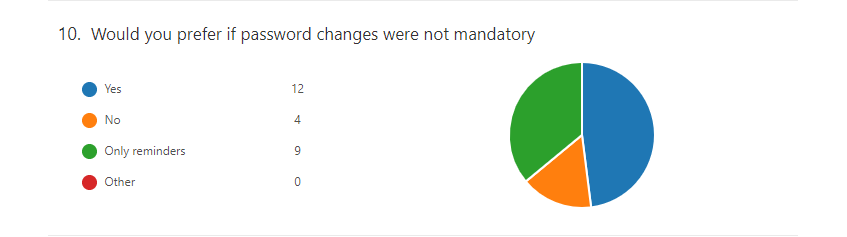
\includegraphics[width=\textwidth]{survey/10.png}
    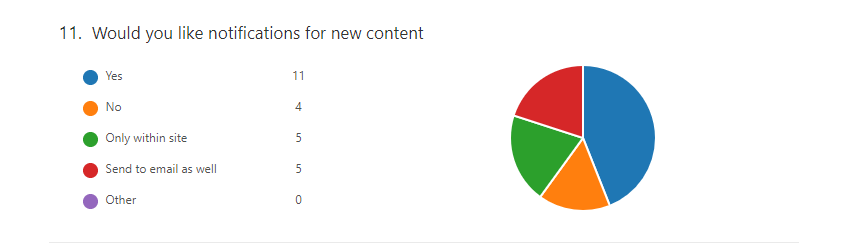
\includegraphics[width=\textwidth]{survey/11.png}
    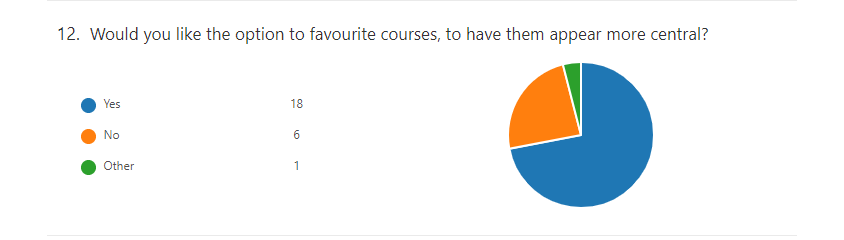
\includegraphics[width=\textwidth]{survey/12.png}

    \paragraph{}
    To view the survey, go to http://lms.survey.giammar.co and to see the up-to-date\\responses, go to http://lms.results.giammar.co

    \section{User Goals}\label{sec:user-goals}

    According to the survey there are many things that are important across a large amount of the people surveyed.
    We can take these things to be the main common goals of the users and what they are looking for.
    It is important to users that there are a place for announcements, a way for the instructor to make a bulletin for all individuals within the class, with possible notifications for such.
    Grade reporting is a must, as it allows the user to evaluate their success within the class and how to move forward with unexpected results.
    A place for class documents is important, as a way for the instructor to upload class information including lecture slides and syllabus and miscellaneous other documents.
    A way for assignments to be submitted online, with a central location across all courses.
    A calendar with important dates for all courses the individual is enrolled in would make the experience much nicer.
    Direct communication toward the professor and/or teacher assistants within the app would be a nice add.
    A better unified user experience between courses and content would make the lives of the users better.


    \section{User Persona}\label{sec:user-persona}

    %todo Me


    \section{Presentation}\label{sec:presentation}

    The content will be displayed as a web app.
    This allows the content to be viewable on a wide range of devices including mobile and desktop.
    Since this is a web app, it will reflow intelligently for the device it is being used on.

    If there is sufficent demand, the app can be bundled into 'native' applications using the web app ui.


    \section{Storyboard}\label{sec:storyboard}

    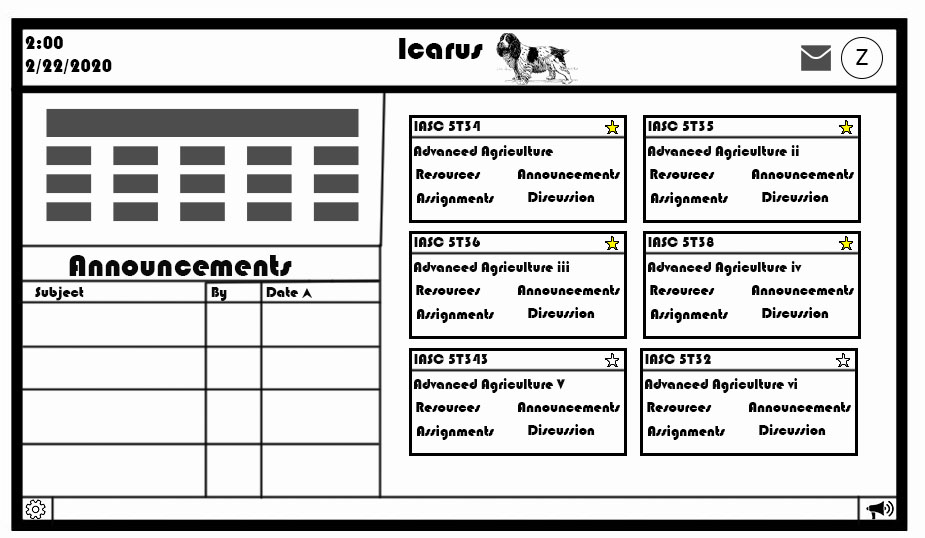
\includegraphics[width=\textwidth]{StoryBoard.jpg}

\end{document}